%%%%%%%%%%%%%%%%%%%%%%%%%%%%%%%%%%%%%%%%%%%%%%%%%%%%%%%%%%%%
%% DISE�O
%%%%%%%%%%%%%%%%%%%%%%%%%%%%%%%%%%%%%%%%%%%%%%%%%%%%%%%%%%%%


El software estar�a compuesto por tres m�dulos independientes. Un m�dulo \textit{Core}, un m�dulo \textit{RAL} y un m�dulo \textit{GUI}.
Esto nos permite realizar el desarrollo de cada m�dulo completamente por separado.



Algo as� como la Figura \ref{Fig:arq}:

\begin{figure}
	\centering
	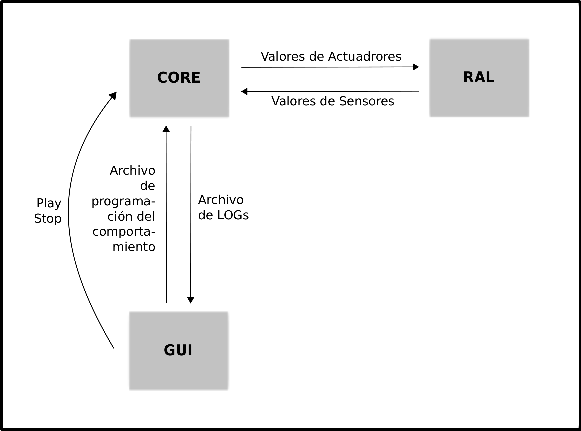
\includegraphics[scale=0.7]{images/arquitectura.png}
	\caption{ERBPI ARQUITECTURA.}
	\label{Fig:arq}
\end{figure}


ARREGLAR ESTO, COMPLETAR CON LO DEL EUROBOT2011 QUE EST\'A MUY BIEN...